\FloatBarrier
\clearpage
\onecolumn
\appendix

\begin{center}
{\Large \textbf{APPENDIX}}
\end{center}

\section{Supplementary Material}
\label{sec:appendix}

This appendix provides (A.1) team contributions, (A.2) reproducibility details, (A.3) additional
predictive, faithfulness and subgroup results, (A.4) additional human-study results, (A.5) qualitative
coding results, (A.6) the legal context and (A.7) the local research interface.

\subsection{Team Contributions}
\label{sec:app-contrib}

\begin{table}[H]
\centering
\caption{Main contributions of each team member.}
\label{tab:contributions}
\footnotesize
\begin{tabular}{@{}p{4.6cm}p{11.0cm}@{}}
\toprule
\textbf{Member} & \textbf{Contributions} \\
\midrule
Aye Khin Khin Hpone (Yolanda Lim) & Modelling pipeline, frozen protocol, one-time final test and model card; study cases, explanation charts and human-study analysis; sensitivity analyses; local research interface with what-if mode; integration, verification and reproducibility of all workstreams \\
Nguyen Liem Son (Lucas) & Seeded participant-assignment generator; explanation-chart and profile-card renderer with answer-leak check; unit tests and documentation for both \\
Witchayda Theppithuk (Noey) & Validation data and model-evaluation audits; full explanation audit on 544 validation students (faithfulness, stability, pair masking, surrogates and recourse); topic analyses, audit figures and results notebooks \\
Han Htoo Zaw (Han) & Google Forms specification, generator and Apps Script renderer; case-pack contract; response transformation; live form build, privacy settings and export checks \\
Pyae Sone Han (Harry) & Consent, instructions, debrief and retention arrangements; recruitment coordination; pilot; participant send log and data collection \\
\midrule
All members & Recruitment of about ten participants each; report and presentation \\
\bottomrule
\end{tabular}
\end{table}

\subsection{Reproducibility and Provenance}
\label{sec:app-repro}

The split row identifiers, protocol, code snapshot and fitted model were hashed before the final
test, and a lock file records that the test was run once (2 November 2026) and never repeated. The
same final-test pipeline was first rehearsed on the validation split (saved separately as a dry run),
and automated data checks on all 544 validation records found no non-finite values, impossible unit
counts, out-of-range grades or duplicate profiles. All
report numbers are regenerated from saved aggregate outputs with \texttt{python
scripts/build\_report\_assets.py}, and \texttt{python scripts/verify\_release\_readiness.py} checks
them against the saved evidence without fitting models or reading the test split. Raw survey
responses, participant codes and the case-to-answer lookup are kept outside the repository, and only
aggregate tables are shared. The repository separates source data, exploratory analysis, modelling,
explanation evaluation, study materials and outputs; a pinned Python 3.12 environment and seed 42
support a fresh clone, \texttt{python scripts/launch\_interface.py} builds the local interface, and a
model card (intended use, data, final metrics, explanation evidence, subgroup results and
limitations) is included in the project handoff document (\texttt{docs/HANDOFF.md}, Section~8).
The test suite (98 unit tests) covers the modelling, explanation, study-integrity, interface and
report-tooling code.

\subsection{Additional Predictive, Faithfulness and Subgroup Results}
\label{sec:app-pred}

\begin{figure}[tbp]
\centering
\begin{minipage}[b]{0.48\linewidth}\centering
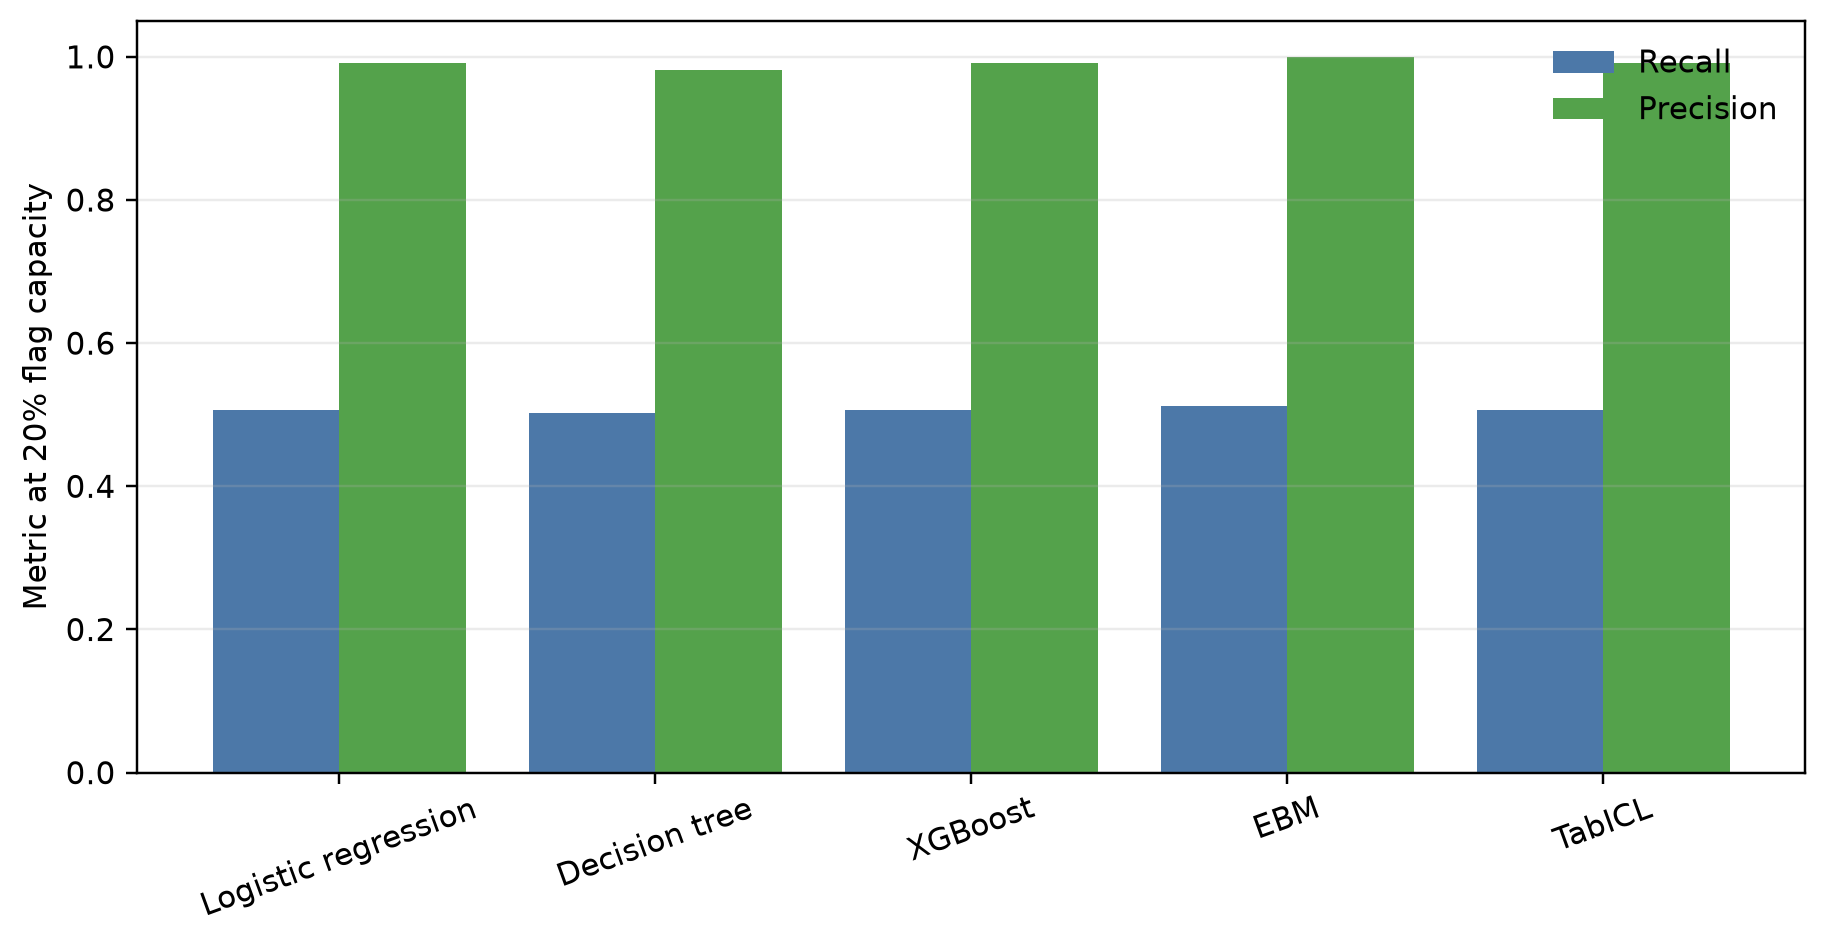
\includegraphics[width=\linewidth]{final_test_outreach_metrics.png}\\[2pt]
{\small (a) Final-test recall and precision at 20\% capacity}
\end{minipage}\hfill
\begin{minipage}[b]{0.48\linewidth}\centering
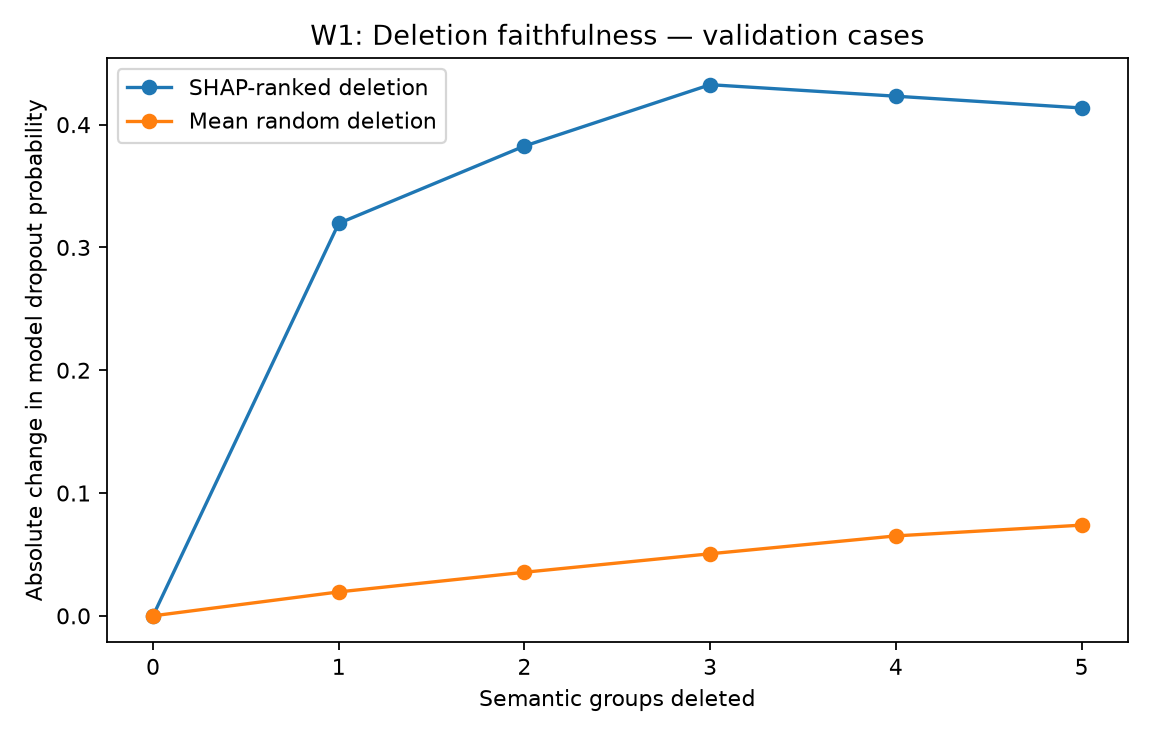
\includegraphics[width=\linewidth,trim=0 0 0 25,clip]{deletion_faithfulness_validation.png}\\[2pt]
{\small (b) Faithfulness on 544 validation students}
\end{minipage}
\caption{Capacity-limited recall and precision (a) and deletion faithfulness (b).}
\label{fig:outreach}
\label{fig:faithfulness}
\end{figure}

With 109 slots and 213 test dropouts, recall cannot exceed 0.51 (Figure~\ref{fig:outreach}a), and
removing groups in SHAP order moves the prediction far more than removing them in random order
(Figure~\ref{fig:faithfulness}b). Table~\ref{tab:subgroups} reports final-test subgroups (left) and
validation recall with and without protected attributes (right); gender follows the UCI coding
(0 = female).

\textbf{Global explanations.} Three global views agree with the local SHAP ranking. Grouped
permutation importance on 100 validation students (5 repeats) ranks first-semester progress far
ahead (ROC-AUC loss 0.255), followed by tuition fees (0.038) and participation (0.025); every other
group costs less than 0.005. The independently fitted EBM gives its largest mean contributions to
first-semester pass rate, tuition fees, course, first-semester grade and scholarship status. ALE
curves for admission grade, age at enrolment and credited units stay within $\pm0.03$ of the average
prediction, so these inputs move the estimate little once first-semester results are known.

\textbf{Pairwise masking.} Masking pairs of each student's top five groups jointly rather than
separately shows a mean absolute non-additive response of 0.036 probability units; the largest common
pair is first-semester progress with participation (0.197 across 320 students). Adding pair terms
reduced the local surrogate error from 0.073 to 0.022 for lasso (pair surrogates were better for
95\% of students), so the five bars, read as separate effects, understate how these two
first-semester groups act together.

\begin{table}[H]
\centering
\caption{Validation sensitivity analyses (exploratory; not used for model selection).}
\label{tab:sensitivity}
\footnotesize
\begin{tabular}{@{}lcccc@{}}
\toprule
\textbf{Setting} & \textbf{ROC-AUC} & \textbf{Brier} & \textbf{Recall@20\%} & \textbf{Precision@20\%} \\
\midrule
Primary (after first semester, 33 features) & 0.952 & 0.071 & 0.507 & 1.000 \\
Admission-time window (no first-semester results) & 0.874 & 0.135 & 0.469 & 0.926 \\
Without protected attributes (27 features, refit) & 0.950 & 0.072 & 0.507 & 1.000 \\
Enrolled share added as non-dropout (frozen model) & 0.924 & 0.111 & 0.587 & 0.947 \\
Enrolled share added as non-dropout (grouped refit) & 0.929 & 0.085 & 0.606 & 0.977 \\
Only students with $\geq$1 first-semester evaluation (frozen model, re-ranked) & 0.949 & -- & 0.559 & 1.000 \\
\bottomrule
\end{tabular}
\end{table}

\begin{table}[H]
\centering
\caption{Descriptive subgroup diagnostics (-- = suppressed, fewer than 30).}
\label{tab:subgroups}
\footnotesize
\begin{tabular}{@{}llcccc@{\hspace{18pt}}cc@{}}
\toprule
 & & \multicolumn{4}{c}{\textbf{Final test}} & \multicolumn{2}{c}{\textbf{Validation recall}} \\
\cmidrule(lr){3-6}\cmidrule(l){7-8}
\textbf{Attribute} & \textbf{Group} & \textbf{n} & \textbf{Dropout rate} & \textbf{Flag rate} & \textbf{Recall} & \textbf{All features} & \textbf{No protected} \\
\midrule
Gender & Female & 335 & 0.299 & 0.122 & 0.410 & 0.404 & 0.455 \\
       & Male   & 210 & 0.538 & 0.324 & 0.593 & 0.597 & 0.553 \\
\addlinespace
Displaced & No  & 229 & 0.476 & 0.288 & 0.596 & 0.583 & 0.592 \\
          & Yes & 316 & 0.329 & 0.136 & 0.414 & 0.409 & 0.398 \\
\addlinespace
Age at entry & $\leq$20 & 318 & 0.283 & 0.116 & 0.411 & 0.342 & 0.378 \\
             & 21--25   & 93  & 0.430 & 0.194 & 0.450 & 0.565 & 0.500 \\
             & 26--35   & 83  & 0.663 & 0.434 & 0.655 & 0.632 & 0.632 \\
             & 36+      & 51  & 0.549 & 0.353 & 0.607 & -- & -- \\
\bottomrule
\end{tabular}
\end{table}

\subsection{Additional Human-Study Results}

\begin{figure}[H]
\centering
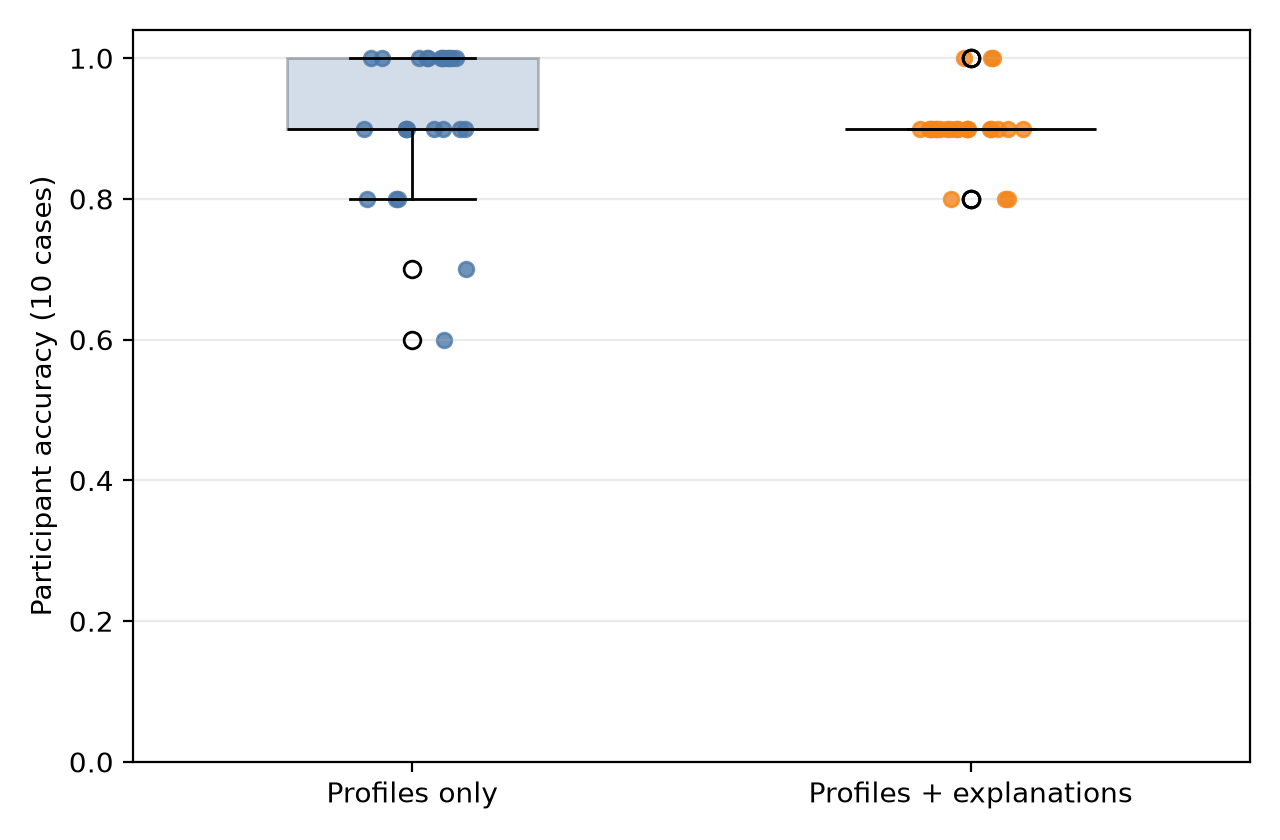
\includegraphics[width=0.40\linewidth]{human_accuracy_by_group.png}\hspace{0.06\linewidth}
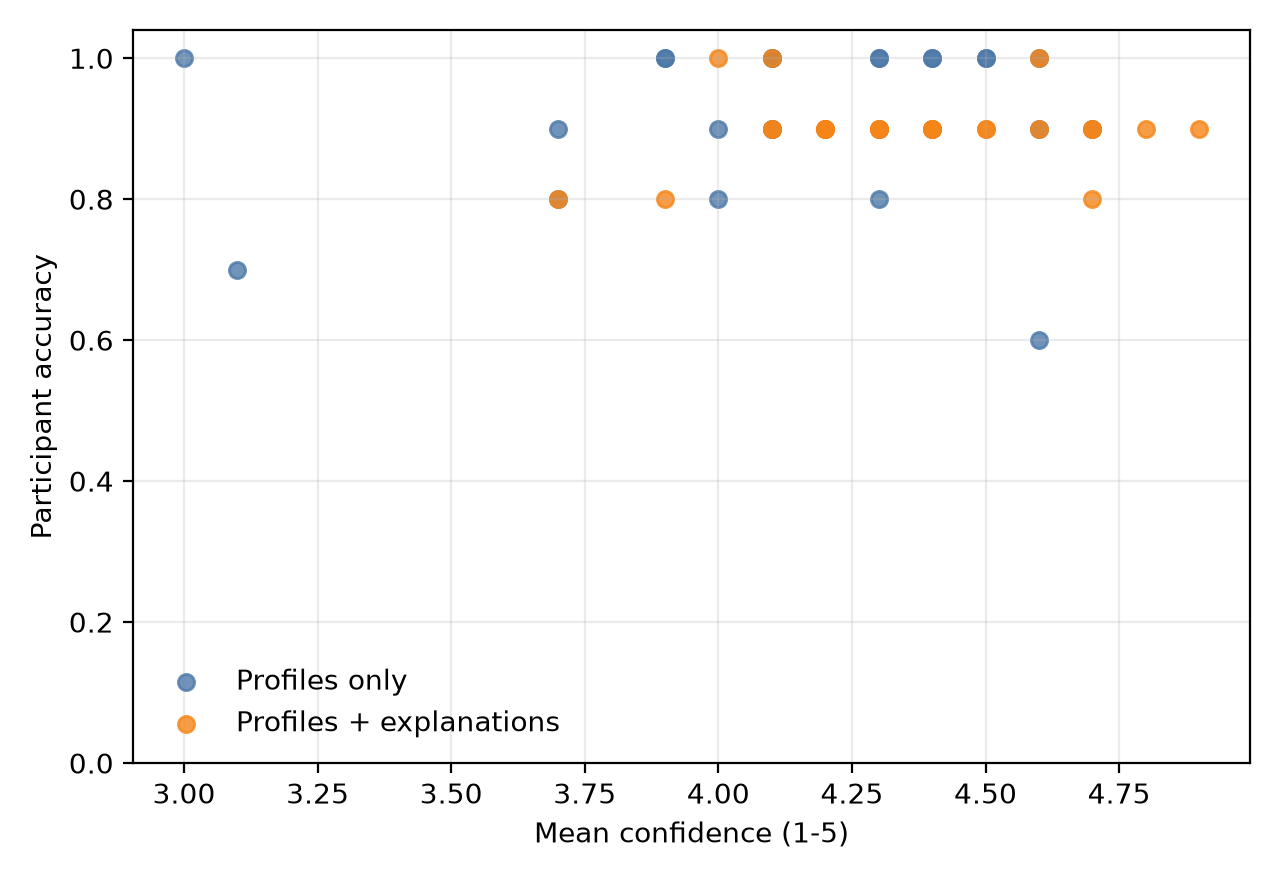
\includegraphics[width=0.40\linewidth]{human_confidence_vs_accuracy.png}\\[4pt]
\makebox[0.40\linewidth]{\small (a) Accuracy by group}\hspace{0.06\linewidth}\makebox[0.40\linewidth]{\small (b) Confidence vs.\ accuracy}
\caption{Participant-level accuracy and confidence.}
\label{fig:human-extra}
\end{figure}

\begin{table}[H]
\centering
\caption{Case-level accuracy and the B $-$ A difference without each case (95\% intervals).}
\label{tab:cases}
\footnotesize
\begin{tabular}{@{}lcccc@{}}
\toprule
\textbf{Case} & \textbf{Model flag} & \textbf{Acc.\ A} & \textbf{Acc.\ B} & \textbf{B $-$ A without this case} \\
\midrule
C01 & No  & 0.60 & 0.20 & $+$0.027 [$-$0.013, 0.076] \\
C02 & No  & 0.96 & 0.96 & $-$0.018 [$-$0.062, 0.036] \\
C03 & No  & 0.96 & 0.96 & $-$0.018 [$-$0.062, 0.031] \\
C04 & No  & 0.96 & 1.00 & $-$0.022 [$-$0.067, 0.031] \\
C05 & Yes & 0.96 & 0.96 & $-$0.018 [$-$0.062, 0.027] \\
C06 & Yes & 0.96 & 1.00 & $-$0.022 [$-$0.067, 0.027] \\
C07 & No  & 0.84 & 0.92 & $-$0.027 [$-$0.067, 0.013] \\
C08 & Yes & 0.96 & 1.00 & $-$0.022 [$-$0.067, 0.027] \\
C09 & Yes & 1.00 & 1.00 & $-$0.018 [$-$0.067, 0.036] \\
C10 & Yes & 0.96 & 1.00 & $-$0.022 [$-$0.071, 0.031] \\
\bottomrule
\end{tabular}
\end{table}

\subsection{Qualitative Coding Results}

\begin{table}[H]
\centering
\caption{Primary themes of the 1,500 written answers (single coding pass).}
\label{tab:themes}
\footnotesize
\begin{tabular}{@{}llr@{\hspace{24pt}}llr@{}}
\toprule
\textbf{Question} & \textbf{Theme} & \textbf{\%} & \textbf{Question} & \textbf{Theme} & \textbf{\%} \\
\midrule
Why flagged & Explanation chart & 36.0 & Suggested support & Academic support & 29.8 \\
 & Academic evidence & 31.0 & & No action & 21.0 \\
 & Several factors & 28.0 & & Advising or monitoring & 16.0 \\
 & Financial or admin. & 3.0 & & Financial or admin.\ support & 15.2 \\
 & Other & 2.0 & & Verify information first & 11.4 \\
\cmidrule{4-6}
 & & & Missing information & Academic engagement & 39.8 \\
 & & & & Personal circumstances & 25.8 \\
 & & & & Course or institution & 12.0 \\
 & & & & Finances & 9.8 \\
 & & & & Nothing / unclear & 12.4 \\
\bottomrule
\end{tabular}
\end{table}

\subsection{Legal Context}
\label{sec:app-legal}

No formal legal review was carried out; this section indicates which data-protection rules would be
relevant if the approach were taken further. The UCI dataset is anonymised and public, so the
modelling itself processes no personal data. The participant responses are pseudonymous rather than
anonymous while the case-linkage files exist, and would count as personal data under both the EU
General Data Protection Regulation (GDPR)~\citep{gdpr2016} and Thailand's Personal Data Protection
Act (PDPA)~\citep{pdpa2019}. Both laws rest on a lawful basis such as consent, purpose limitation,
data minimisation and security, which the study addressed through informed consent, no names, random
codes, restricted access and use for this course project only.

A deployed outreach system would raise further obligations. Real student records are personal data,
and attributes such as health or special needs may be sensitive data requiring stronger safeguards.
GDPR Article~22 restricts decisions based solely on automated processing that significantly affect a
person~\citep{gdpr2016,wachter2017counterfactual}; the outreach rule in this report keeps an adviser
responsible for every contact and never withholds support, but an institution would still need to
inform students, assess the data-protection impact and confirm the rules of its own jurisdiction
before any use.

\subsection{Local Research Interface}
\label{sec:app-interface}

To illustrate how the outputs could reach a support officer, a self-contained local web page was
built for the 543 validation students not used in the study (Figure~\ref{fig:interface}). For each
student, it shows whether the student would be flagged and their rank on the cohort risk curve, the
five largest grouped contributions, the stability of that explanation, the fee/debt recourse check
(labelled as model behaviour rather than advice) and the profile. An optional local what-if mode
re-scores an edited copy of a student with the frozen model, allowing changes to first-semester
results and fee, debt or scholarship status only. It keeps the other 543 scores fixed, rejects
impossible combinations (for example, more units passed than enrolled) and reproduced all 104 saved
fee/debt scenarios (largest probability difference $4.1\times10^{-6}$, identical ranks).
Figure~\ref{fig:interface}(b) applies it to a flagged student: clearing the unpaid fees and the debt
lowers the estimate from 0.996 to 0.689 and the rank from 87 to 182, so the student would no longer be
flagged. Such results describe how the model responds, not what would happen to the student. The
interface was built after the study, uses validation data only, runs solely on the local machine and
was not tested with users; it is therefore a demonstration rather than evidence.

\begin{figure}[tbp]
\centering
\begin{minipage}[t]{0.47\linewidth}\vspace{0pt}\centering
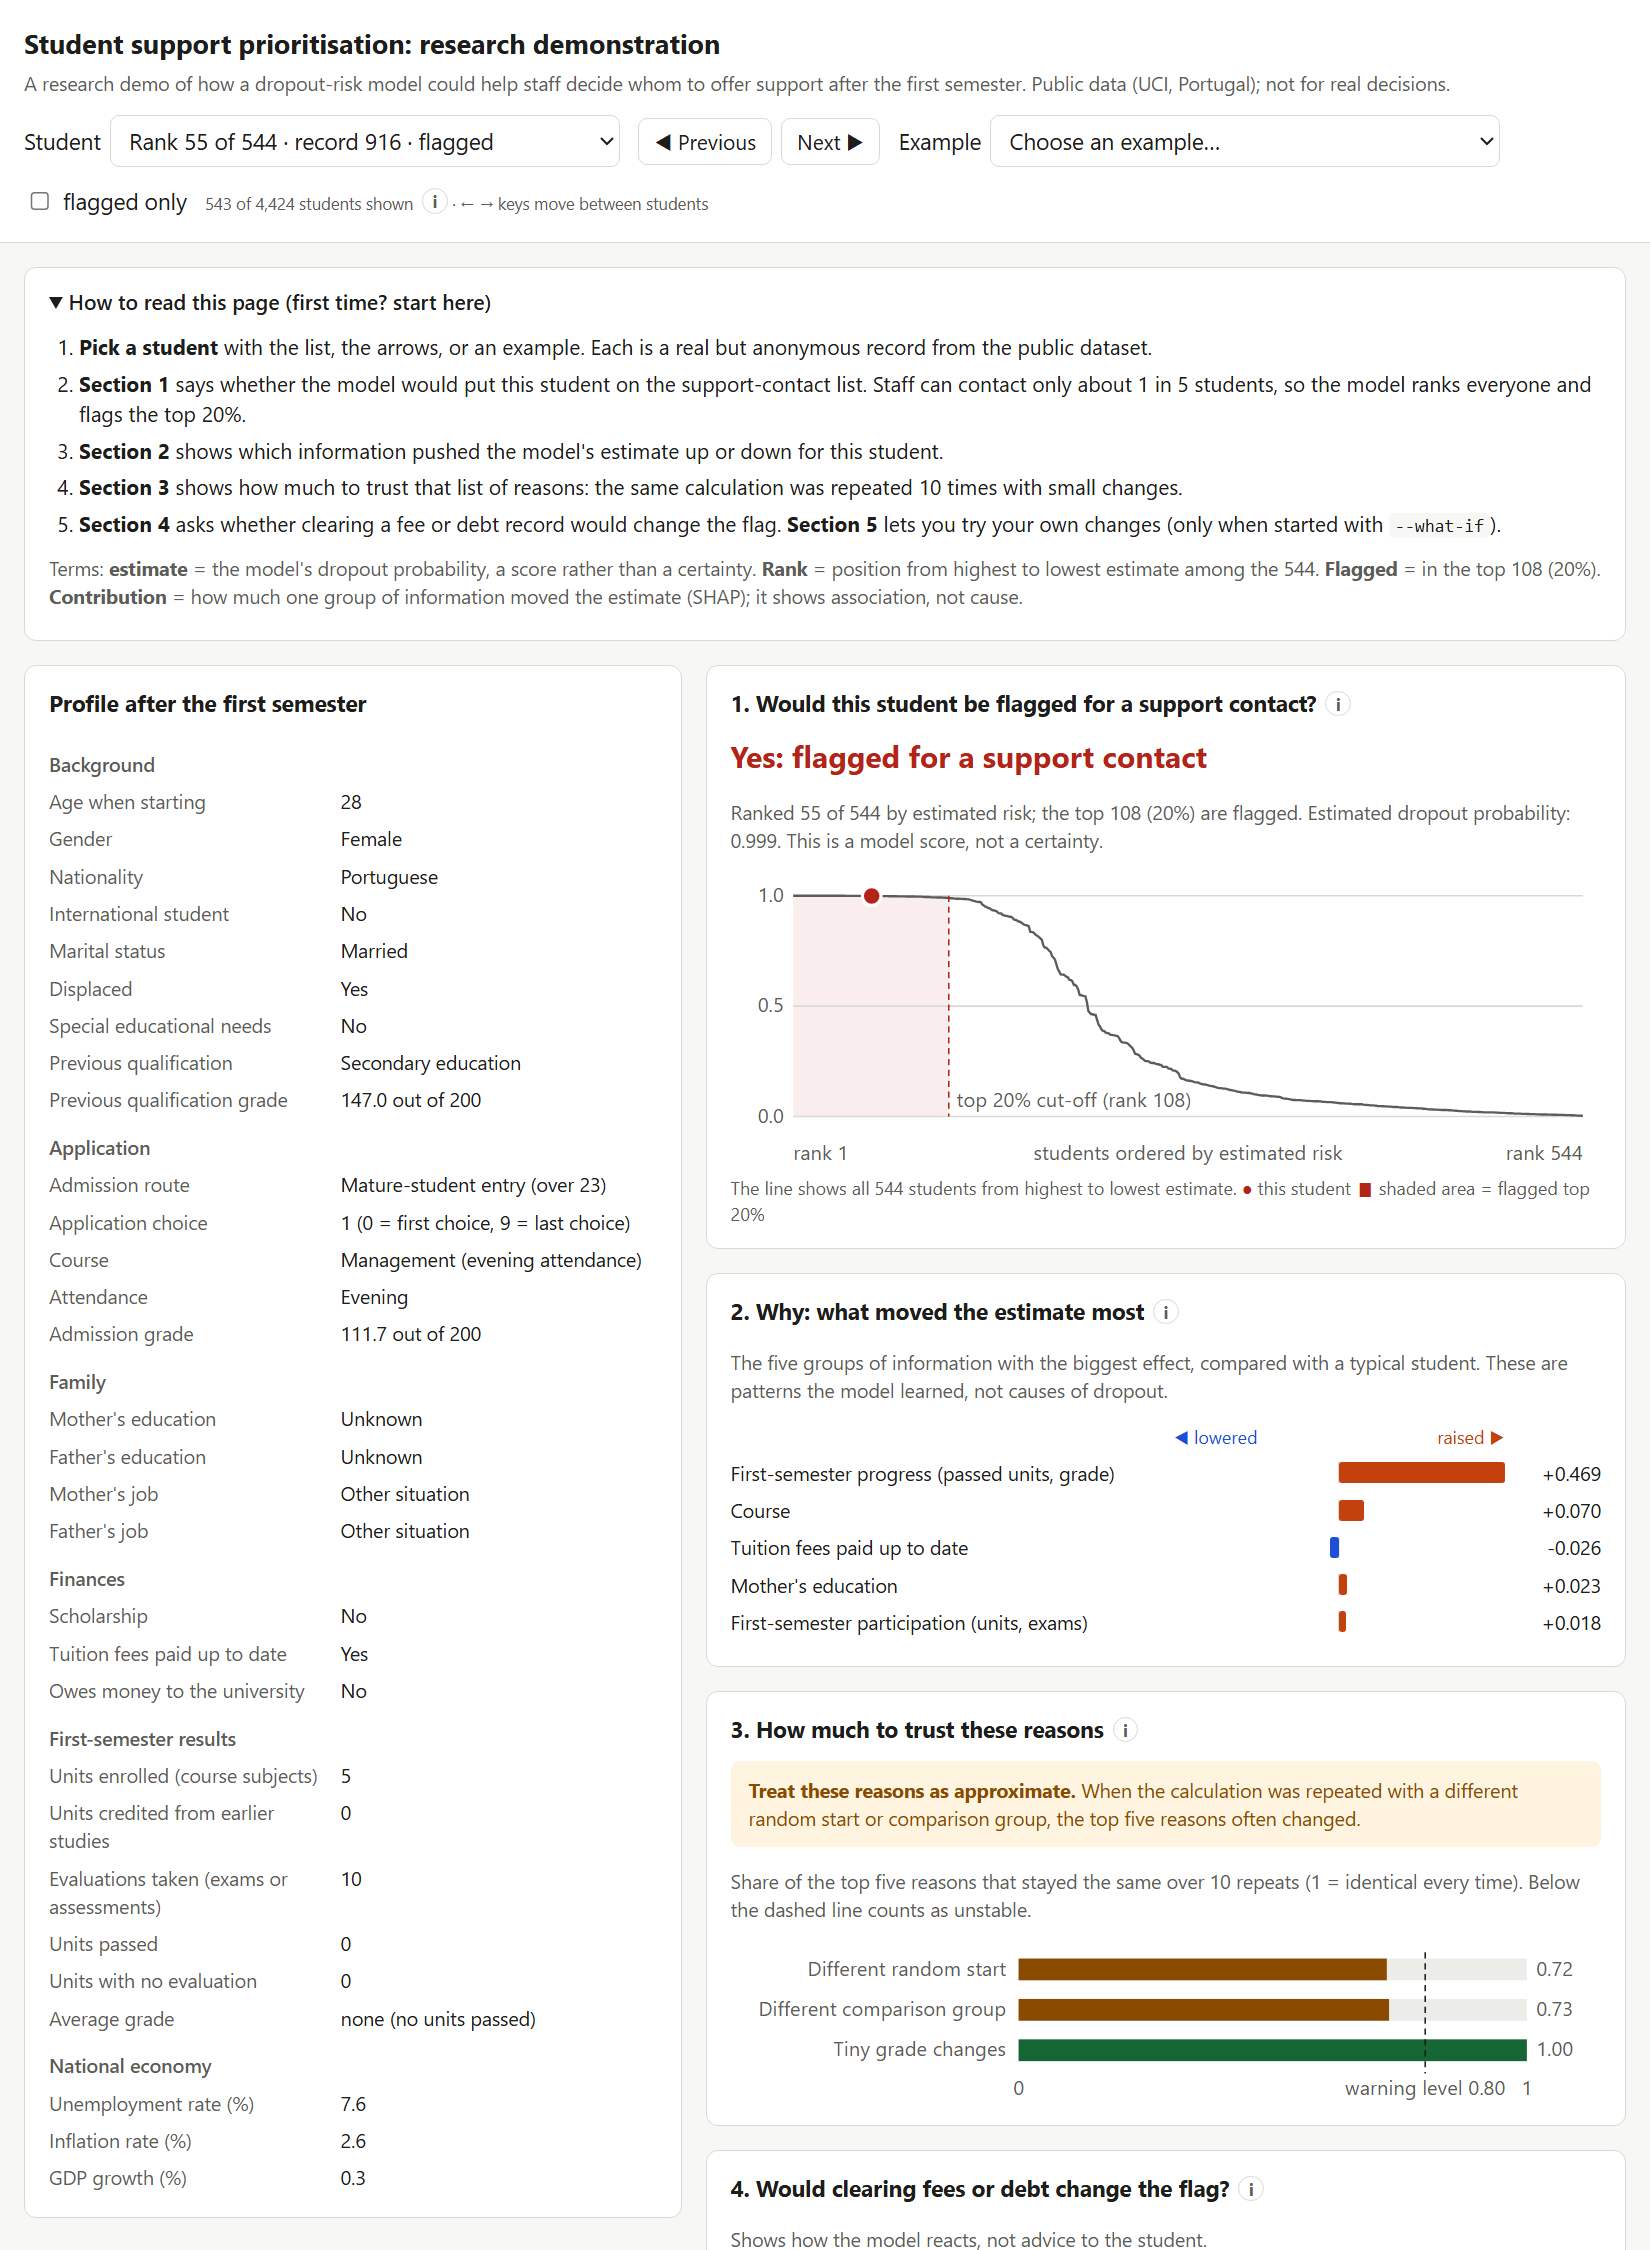
\includegraphics[height=0.43\textheight]{figures/interface_validation_916.png}\\[2pt]
{\small (a) Saved view: flag, rank, reasons and their stability}
\end{minipage}\hfill
\begin{minipage}[t]{0.51\linewidth}\vspace{0pt}\centering
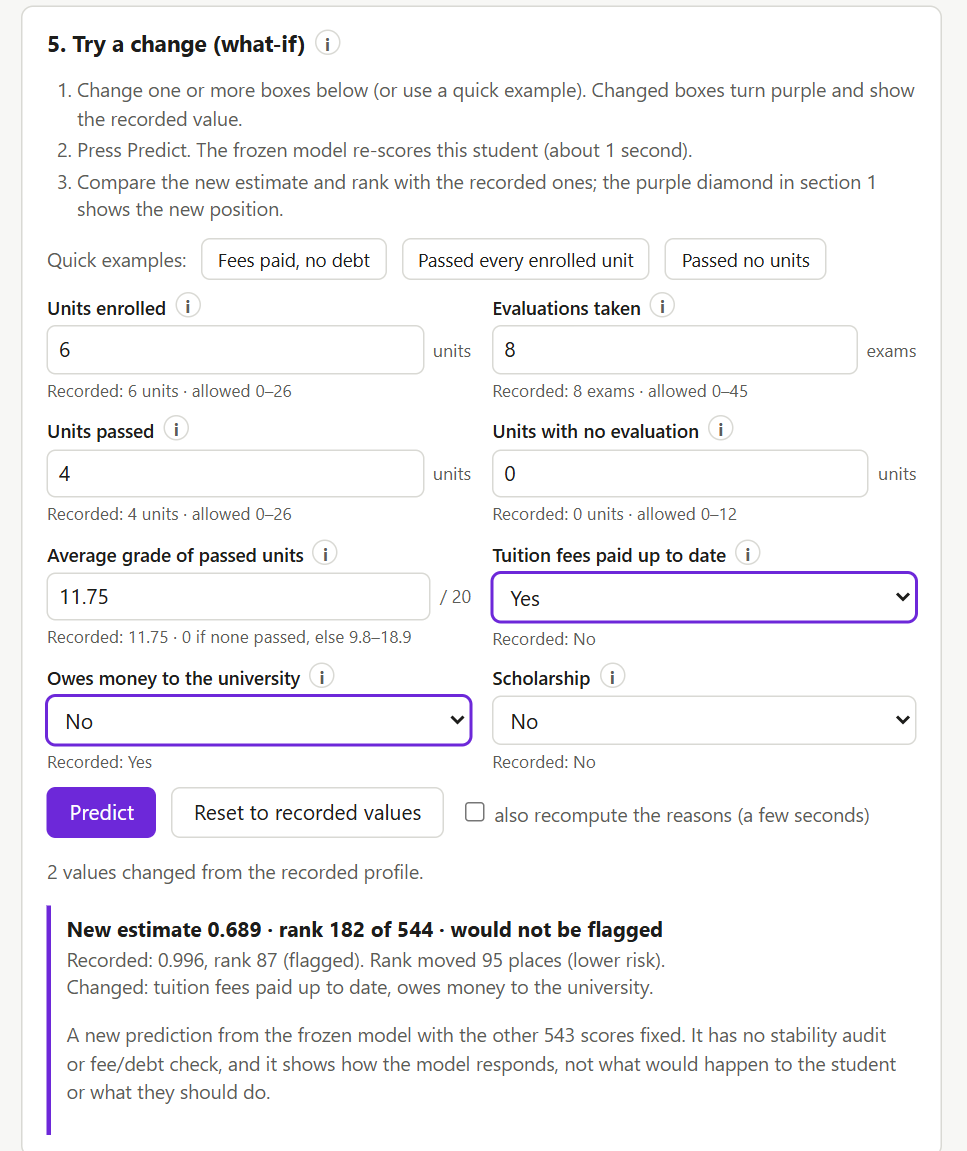
\includegraphics[height=0.43\textheight]{figures/interface_whatif_174.png}\\[2pt]
{\small (b) What-if mode: fees paid and debt cleared}
\end{minipage}
\caption{Local research interface (validation students only): (a) saved view for student 916; (b) what-if mode for student 174.}
\label{fig:interface}
\end{figure}
